\documentclass[11pt,t]{beamer}
% xcolor and define colors -------------------------
\usepackage{xcolor}

% https://www.viget.com/articles/color-contrast/
\definecolor{purple}{HTML}{695693}
\definecolor{navy}{HTML}{567293}
\definecolor{ruby}{HTML}{9a2515}
\definecolor{alice}{HTML}{107895}
\definecolor{daisy}{HTML}{EBC944}
\definecolor{coral}{HTML}{F26D21}
\definecolor{kelly}{HTML}{829356}
\definecolor{cranberry}{HTML}{E64173}
\definecolor{jet}{HTML}{131516}
\definecolor{asher}{HTML}{555F61}
\definecolor{slate}{HTML}{314F4F}

% Main theme colors
\definecolor{accent}{HTML}{107895}
\definecolor{accent2}{HTML}{9a2515}

\newcommand\navy[1]{{\color{navy}#1}}
\newcommand\purple[1]{{\color{purple}#1}}
\newcommand\kelly[1]{{\color{kelly}#1}}
\newcommand\ruby[1]{{\color{ruby}#1}}
\newcommand\alice[1]{{\color{alice}#1}}
\newcommand\daisy[1]{{\color{daisy}#1}}
\newcommand\coral[1]{{\color{coral}#1}}
\newcommand\cranberry[1]{{\color{cranberry}#1}}
\newcommand\slate[1]{{\color{slate}#1}}
\newcommand\jet[1]{{\color{jet}#1}}
\newcommand\asher[1]{{\color{asher}#1}}

\newcommand\bgNavy[1]{{\colorbox{navy!80!white}{\textcolor{white}{#1}}}}
\newcommand\bgPurple[1]{{\colorbox{purple!80!white}{\textcolor{white}{#1}}}}
\newcommand\bgKelly[1]{{\colorbox{kelly!80!white}{\textcolor{white}{#1}}}}
\newcommand\bgRuby[1]{{\colorbox{ruby!80!white}{\textcolor{white}{#1}}}}
\newcommand\bgAlice[1]{{\colorbox{alice!80!white}{\textcolor{white}{#1}}}}
\newcommand\bgDaisy[1]{{\colorbox{daisy!80!white}{\textcolor{white}{#1}}}}
\newcommand\bgCoral[1]{{\colorbox{coral!80!white}{\textcolor{white}{#1}}}}
\newcommand\bgCranberry[1]{{\colorbox{cranberry!80!white}{\textcolor{white}{#1}}}}


% Beamer Options -------------------------------------

% Background
\setbeamercolor{background canvas}{bg = white}

% Change text margins
\setbeamersize{text margin left = 15pt, text margin right = 15pt} 

% \alert
\setbeamercolor{alerted text}{fg = accent2}

% Frame title
\setbeamercolor{frametitle}{bg = white, fg = jet}
\setbeamercolor{framesubtitle}{bg = white, fg = accent}
\setbeamerfont{framesubtitle}{size = \small, shape = \itshape}

% Block
\setbeamercolor{block title}{fg = white, bg = accent2}
\setbeamercolor{block body}{fg = jet, bg = jet!10!white}

% Title page
\setbeamercolor{title}{fg = jet}
\setbeamercolor{subtitle}{fg = accent}

%% Custom \maketitle and \titlepage
\setbeamertemplate{title page}
{
    %\begin{centering}
        \vspace{20mm}
        {\Large \usebeamerfont{title}\usebeamercolor[fg]{title}\inserttitle}\\ \vskip0.25em%
        \ifx\insertsubtitle\@empty%
        \else%
          {\usebeamerfont{subtitle}\usebeamercolor[fg]{subtitle}\insertsubtitle\par}%
        \fi% 
        {\vspace{10mm}\insertauthor}\\
        {\color{asher}\small{\insertdate}}\\
    %\end{centering}
}

% Table of Contents
\setbeamercolor{section in toc}{fg = accent!70!jet}
\setbeamercolor{subsection in toc}{fg = jet}

% Button 
\setbeamercolor{button}{bg = accent}

% Remove navigation symbols
\setbeamertemplate{navigation symbols}{}

% Optional: page numbers at bottom
\addtobeamertemplate{navigation symbols}{}{%
    \usebeamerfont{footline}%
    \hspace{1em}%
    \alice{\insertframenumber/\inserttotalframenumber}
    \vspace*{1.5mm}
}


% Table and Figure captions
\setbeamercolor{caption}{fg=jet!70!white}
\setbeamercolor{caption name}{fg=jet}
\setbeamerfont{caption name}{shape = \itshape}

% Bullet points

%% Fix left-margins
\settowidth{\leftmargini}{\usebeamertemplate{itemize item}}
\addtolength{\leftmargini}{\labelsep}

%% enumerate item color
\setbeamercolor{enumerate item}{fg = accent}
\setbeamerfont{enumerate item}{size = \small}
\setbeamertemplate{enumerate item}{\insertenumlabel.}

%% enumerate subitem color
\setbeamercolor{enumerate subitem}{fg = accent!60!white}
\setbeamerfont{enumerate subitem}{size = \small}
\setbeamertemplate{enumerate subitem}{\insertenumlabel.}

%% itemize
\setbeamercolor{itemize item}{fg = accent!70!white}
\setbeamerfont{itemize item}{size = \small}
\setbeamertemplate{itemize item}[circle]

%% right arrow for subitems
\setbeamercolor{itemize subitem}{fg = accent!60!white}
\setbeamerfont{itemize subitem}{size = \small}
\setbeamertemplate{itemize subitem}{$\rightarrow$}

\setbeamertemplate{itemize subsubitem}[square]
\setbeamercolor{itemize subsubitem}{fg = jet}
\setbeamerfont{itemize subsubitem}{size = \small}

% References

%% Bibliography Font, roughly matching aea
\setbeamerfont{bibliography item}{size = \footnotesize}
\setbeamerfont{bibliography entry author}{size = \footnotesize, series = \bfseries}
\setbeamerfont{bibliography entry title}{size = \footnotesize}
\setbeamerfont{bibliography entry location}{size = \footnotesize, shape = \itshape}
\setbeamerfont{bibliography entry note}{size = \footnotesize}

\setbeamercolor{bibliography item}{fg = jet}
\setbeamercolor{bibliography entry author}{fg = accent!60!jet}
\setbeamercolor{bibliography entry title}{fg = jet}
\setbeamercolor{bibliography entry location}{fg = jet}
\setbeamercolor{bibliography entry note}{fg = jet}

%% Remove bibliography symbol in slides
\setbeamertemplate{bibliography item}{}





% Links ----------------------------------------------

\usepackage{hyperref}
\hypersetup{
  colorlinks = true,
  linkcolor = accent2,
  filecolor = accent2,
  urlcolor = accent2,
  citecolor = accent2,
}


% Line spacing --------------------------------------
\usepackage{setspace}
% \setdisplayskipstretch{2}
\setstretch{1.3}


% \begin{columns} -----------------------------------
\usepackage{multicol}


% Fonts ---------------------------------------------
% Beamer Option to use custom fonts
\usefonttheme{professionalfonts}

% \usepackage[utopia, smallerops, varg]{newtxmath}
% \usepackage{utopia}
\usepackage[sfdefault,light]{roboto}

% Small adjustments to text kerning
\usepackage{microtype}



% Remove annoying over-full box warnings -----------
\vfuzz2pt 
\hfuzz2pt


% Table of Contents with Sections
\setbeamerfont{myTOC}{series=\bfseries, size=\Large}
\AtBeginSection[]{
        \frame{
            \frametitle{Roadmap}
            \tableofcontents[current]   
        }
    }


% References ----------------------------------------
\usepackage[
    citestyle= authoryear,
    style = authoryear,
    natbib = true, 
    backend = biber
]{biblatex}

% Smaller font-size for references
\renewcommand*{\bibfont}{\small}

% Remove "In:"
\renewbibmacro{in:}{}

% Color citations for slides
\newenvironment{citecolor}
    {\footnotesize\begin{color}{accent2}}
    {\end{color}}

\newcommand{\citetcolor}[1]{{\footnotesize\textcolor{gray}{\citet{#1}}}}
\newcommand{\citepcolor}[1]{{\footnotesize\textcolor{gray}{\citep{#1}}}}

% Tables -------------------------------------------
% Tables too big
% \begin{adjustbox}{width = 1.2\textwidth, center}
\usepackage{adjustbox}
\usepackage{array}
\usepackage{threeparttable, booktabs, adjustbox}
    
% Fix \input with tables
% \input fails when \\ is at end of external .tex file

\makeatletter
\let\input\@@input
\makeatother

% Tables too narrow
% \begin{tabularx}{\linewidth}{cols}
% col-types: X - center, L - left, R -right
% Relative scale: >{\hsize=.8\hsize}X/L/R
\usepackage{tabularx}
\newcolumntype{L}{>{\raggedright\arraybackslash}X}
\newcolumntype{R}{>{\raggedleft\arraybackslash}X}
\newcolumntype{C}{>{\centering\arraybackslash}X}

% Figures

% \imageframe{img_name} -----------------------------
% from https://github.com/mattjetwell/cousteau
\newcommand{\imageframe}[1]{%
    \begin{frame}[plain]
        \begin{tikzpicture}[remember picture, overlay]
            \node[at = (current page.center), xshift = 0cm] (cover) {%
                \includegraphics[keepaspectratio, width=\paperwidth, height=\paperheight]{#1}
            };
        \end{tikzpicture}
    \end{frame}%
}

% subfigures
\usepackage{subfigure}

% Strikeout text
\usepackage{cancel}

% Highlight slide -----------------------------------
% \begin{transitionframe} Text \end{transitionframe}
% from paulgp's beamer tips
\newenvironment{transitionframe}{
    \setbeamercolor{background canvas}{bg=accent!60!black}
    \begin{frame}\color{accent!10!white}\LARGE\centering
}{
    \end{frame}
}


% Table Highlighting --------------------------------
% Create top-left and bottom-right markets in tabular cells with a unique matching id and these commands will outline those cells
\usepackage[beamer,customcolors]{hf-tikz}
\usetikzlibrary{calc,fit,shapes.misc,backgrounds}
\usepackage{pgfplots}
\pgfplotsset{compat = newest}
\usetikzlibrary{positioning, arrows.meta}
\usepgfplotslibrary{fillbetween}

% halo around text
%https://tex.stackexchange.com/questions/18472/tikz-halo-around-text
\usepackage[outline]{contour} 
\contourlength{1.2pt}
\tikzset{
  contour text/.style={node contents={\contour{white}{#1}}},
  halo text node/.style={circle, draw, pattern=north east lines}
}


\def\arraystretch{0.75}

% To set the hypothesis highlighting boxes red.
\newcommand\marktopleft[1]{%
    \tikz[overlay,remember picture] 
        \node (marker-#1-a) at (0,1.5ex) {};%
}
\newcommand\markbottomright[1]{%
    \tikz[overlay,remember picture] 
        \node (marker-#1-b) at (0,0) {};%
    \tikz[accent!80!jet, ultra thick, overlay, remember picture, inner sep=4pt]
        \node[draw, rectangle, fit=(marker-#1-a.center) (marker-#1-b.center)] {};%
}


\author{Michael Karas}
\title{Lecture 7  - Cost Minimization}
\subtitle{ECON 3070 - Intermediate Microeconomic Theory}
\date{February X, 2025}

\begin{document}

\begin{frame}
  \titlepage
\end{frame}

\begin{frame}{Overview}
  In the previous lecture,

  \begin{itemize}
    \item We looked at production functions, and how they can be used to represent the relationship between quantity of inputs used, and quantity of output produced.

    \item We also considered how the level of output varies when we vary the quantity of one or all of the inputs.
  \end{itemize}
\end{frame}

\begin{frame}{Overview}
  In this chapter, we will discuss how a firm might choose the mix of inputs that it uses to produce a given level of output, given the prices of those inputs.

  \begin{itemize}
    \item We will also analyze how changes in the prices of those inputs might impact the firm's decision.

    \item Finally, we will consider how the firm's problem varies between the short run and the long run.
  \end{itemize}
\end{frame}


\begin{frame}{Cost Minimization}
  Let's assume for the moment that a firm has decided to produce $Q$ units of output. (We will consider in future lectures how they might choose $Q$.)

  \bigskip
  Then a firm which seeks to generate as much profits as possible will be concerned with producing that output at the lowest cost.

  \pause\bigskip
  \begin{itemize}
    \item The problem of finding the lowest-cost mix of inputs that produces a given level of output is the \textbf{cost-minimization problem}.
  \end{itemize}
\end{frame}

\begin{frame}{Cost Minimization}
  For now, let's assume that the firm uses only labor $(L)$, and capital $(K)$, in production (just like consumers only chosing between two goods)

  \bigskip
  \begin{itemize}
    \item Each input has a price. The price of a unit of labor is called the wage rate $(w)$. The price of a unit of capital services is the rental rate of capital $(r)$.

    \item These prices will affect the amount of labor and capital that a firm chooses to use in production.
  \end{itemize}
\end{frame}

\begin{frame}{Cost Minimization}
  \bigskip

  Note that costs may be implicit or explicit, or both.

  \bigskip
  \textbf{Explicit costs} - Costs that involve outlays of money.

  \begin{itemize}
    \item Examples: Wages, rental fees for capital
  \end{itemize}

  \bigskip
  \textbf{Implicit costs} - Costs that \textit{do not} involve outlays of money

  \begin{itemize}
    \item Examples: Forgone earnings by owner, forgone rental fees on office building
  \end{itemize}
\end{frame}

\begin{frame}{Opportunity Cost}
  \textbf{Opportunity cost} is the value of a sacrificed opportunity.

  \bigskip
  \begin{itemize}
    \item Example: You quit your job as a corporate lawer and start a plumbing business.
  
    \item If your salary before you quit was \$150K per year, then the opportunity cost of the plumbing business is \$150K.
  \end{itemize}
\end{frame}

\begin{frame}{Economic \& Accounting Costs}
  \textbf{Economic costs} are all relevant explicit and implicit costs.

  \begin{itemize}
    \item If you use your office building instead of renting it, the foregone rent is part of your economic cost.
    
    \item `Hidden' (implicit) costs are often why people make decisions, so look out for these everywhere!
  \end{itemize}

  \bigskip
  \textbf{Accounting costs} are simply your explicit costs (wages, rent payments, etc...)
\end{frame}

\begin{frame}{Isocost Lines}
  Before we look at the cost minimization problem mathematically, let's think about it graphically.

  \bigskip
  For this, we will use isocost lines. \textbf{Isocost lines} represent combinations of labor and capital that all have the same \textit{total cost (TC)}.

  \bigskip  
  \begin{itemize}
    \item Total cost is given by $TC = wL + rK$ (similar to the budget line for a consumer).
  \end{itemize}
\end{frame}

\begin{frame}{Isocost Lines}
  Below is a set of isocost lines for a firm, where each line represents a different total cost (TC). Note that as we move northeast in the graph, the isocost lines represent higher and higher total cost levels.

  \begin{figure}
    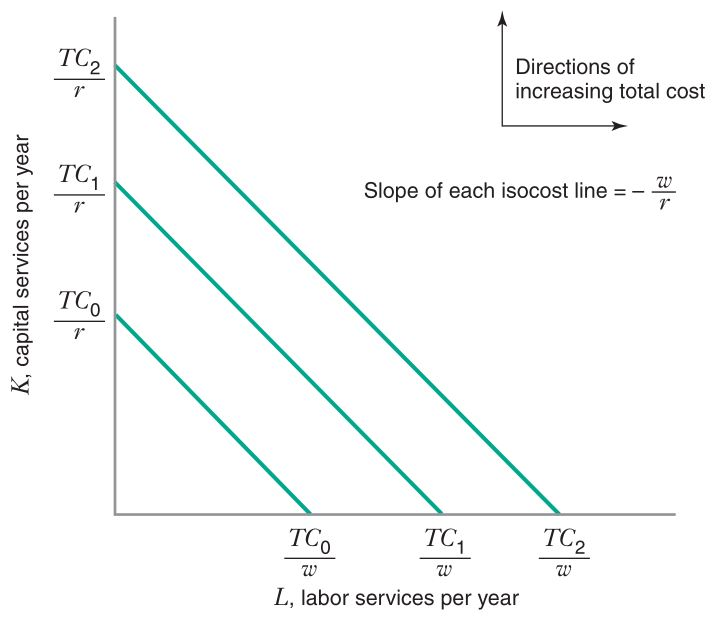
\includegraphics[width=0.55\linewidth]{figures/fig7_1.jpg}
  \end{figure}
\end{frame}

\begin{frame}{Solving the Cost Minimization Problem}
  In general, the cost-minimizing choice of inputs will be the point where the isoquant is just tangent to an isocost line. Consider why that is... \pause

  \begin{itemize}
    \item If the firm chooses a point where the isocost and isoquant lines intersect, but are not tangent, then the firm could, by using more of one input, and less of the other, reduce their cost while still being on that isoquant.
    \item On the other hand, if the firm chooses a point where the isocost and isoquant lines do not touch, then the firm can't feasibly produce the required number of units.
  \end{itemize}
\end{frame}

\begin{frame}{Solving the Cost Minimization Problem}
  \begin{figure}
    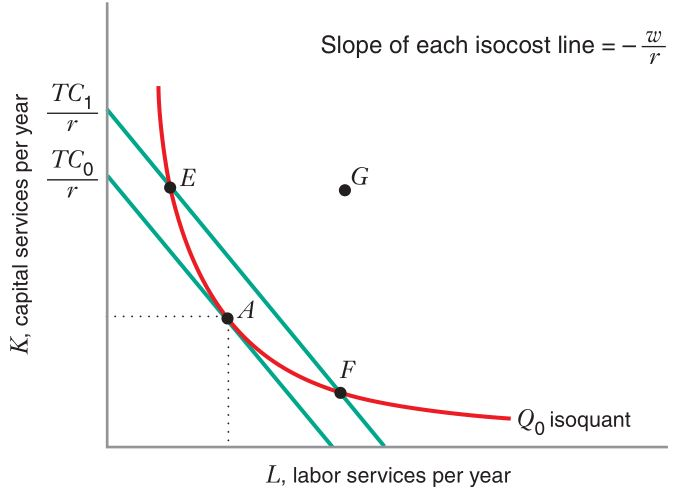
\includegraphics[width=0.8\linewidth]{figures/fig7_2.jpg}
  \end{figure}
\end{frame}



\begin{frame}{The \kelly{Optimality Condition}}
  Just like in the consumer choice setting, the above graph gives us an optimality condition.

  $$
    \kelly{\frac{MP_K}{r} = \frac{MP_L}{w}}
  $$

  \pause\bigskip
  \begin{itemize}
    \item The \kelly{optimality condition} tells us that the produce minimizes cost when the marginal product per dollar on both inputs is equal.
    \item Think about what would happen if it weren't equal for the two inputs.
  \end{itemize}
\end{frame}


\begin{frame}{The Optimality Condition}
  If you were producing the necessary quantity (your constraint!) and 
  $$
    \frac{MP_K}{r} > \frac{MP_L}{w},
  $$
  how could you produce the same quantity and lower costs?

  \pause\bigskip
  Spend $\$1$ less on labor and $<\$1$ more on capital!
\end{frame}

\begin{frame}{The Optimality Condition}
  If you were producing the necessary quantity (your constraint!) and 
  $$
    \frac{MP_K}{r} < \frac{MP_L}{w},
  $$
  how could you produce the same quantity and lower costs?

  \pause\bigskip
  Spend $\$1$ less on capital and $<\$1$ more on labor!
\end{frame}


\begin{frame}{The Optimality Condition}
  Let's double-check that the optimality condition is correct using the Method of Lagrange. Our cost minimization problem can be formally stated as

  $$
    \min_{(K,L)} rK + wL \qquad \text{subject to} \qquad \bar{Q} = Q(K,L)
  $$

  \bigskip
  Our Lagrangian is

  $$
    \mathcal{L}(L,K,\lambda) = rK + wL + \lambda(\bar{Q} - Q(K,L))
  $$
\end{frame}

\begin{frame}{The Optimality Condition}
  The first order conditions for an optimum are:
  \begin{align*}
      & \frac{\delta \mathcal{L}}{\delta K}=0 \Rightarrow r = \lambda(MP_K(K,L))      \\
      & \frac{\delta \mathcal{L}}{\delta L}=0 \Rightarrow w = \lambda(MP_L(K,L)       \\
      & \frac{\delta \mathcal{L}}{\delta \lambda}=0 \Rightarrow \bar{Q} - Q(K,L) = 0
  \end{align*}

  If we solve the first two equations for $\lambda$, and set them equal to each other, we find
  
  $$
    \frac{MP_K}{r} = \frac{MP_L}{w}
  $$
\end{frame}

\begin{frame}{Solving for the Optimal Input Combination}
  Now we have a system of two equations:
  $$
    \frac{MP_K}{r} = \frac{MP_L}{w} \quad\text{and}\quad \bar{Q} = Q(K,L)
  $$

  \bigskip We can solve this system to find the cost-minimizing input combination of $L$ and $K$.
\end{frame}

\begin{frame}{Solving for the Optimal Input Combination}
  Let's look at an example. Suppose a firm wishes to produce 1,000 units of output, and that the prices of labor and capital are \$5 and \$20, respectively. If the firm has the production function\
  $$
    Q = 50 \sqrt{LK}
  $$
  Then,
  $$
    MP_L = 25\sqrt{\tfrac{K}{L}} \quad\text{and}\quad MP_K = 25\sqrt{\tfrac{L}{K}}
  $$
\end{frame}

\begin{frame}{Solving for the Optimal Input Combination}
  Our \kelly{optimality condition} is:
  
  \pause
  $$
    \frac{25\sqrt{K/L}}{5} = \frac{25\sqrt{L/K}}{20} \implies 4K = L
  $$

  \bigskip
  Our constraint of producing 1,000 units is:
  
  \pause
  $$
    1000 = 50 \sqrt{LK}
  $$
\end{frame}

\begin{frame}{Solving for the Optimal Input Combination}
  Our constraint can be simplified to
  $$
    1000 = 50 \sqrt{LK} \implies 400 = LK
  $$

  \pause\bigskip
  If we plug in $L = 4K$, then do some algebra
  \pause
  \begin{equation*}
    K^* = 10 \qquad \text{and} \qquad L^* = 40
  \end{equation*}
\end{frame}


\begin{frame}{Solving for the Optimal Input Combination}
  Suppose instead we just wanted to find  $K^*$ and $L^*$ as functions of $\bar{Q}$, $w$ and $r$. Then our optimality condition is:
  $$
    \frac{25\sqrt{K/L}}{25\sqrt{L/K}}=\frac{w}{r}
    \text{ or } \qquad \frac{K}{L}=\frac{w}{r}
  $$

  \bigskip
  If we rearrange this equation, then:
  $$ 
    K = \frac{w}{r}L
  $$ 
\end{frame}

\begin{frame}{Solving for the Optimal Input Combination}
Combining this with our output quota:
\begin{align*}
  \bar{Q} &= 50\sqrt{LK}             \\
          &= 50\sqrt{\tfrac{w}{r}L^2} \\
          &= 50\sqrt{\tfrac{w}{r}}L
\end{align*}
\end{frame}

\begin{frame}{Solving for the Optimal Input Combination}
  If we solve the previous equation for L:
  \begin{equation*}
    L^*(w,r,\bar{Q})=\frac{\bar{Q}}{50}\sqrt{\tfrac{r}{w}}
  \end{equation*}

  \pause\bigskip
  Then
  \begin{equation*}
    K^*(w,r,\bar{Q}) =\frac{\bar{Q}}{50}\sqrt{\tfrac{w}{r}}
  \end{equation*}

  \bigskip
  These are the \textbf{conditional demand equations} for labor and capital, respectively.
\end{frame}

\begin{frame}{The Total Cost Function}
  Suppose that, now that we have the conditional demand equations, and we want to find the total cost function.

  \pause\bigskip
  Remember that the total cost function is $TC = wL + rK$. We can then plug in our functions for $L^*$ and $K^*$.

  \vspace*{-5mm}
  \begin{align*}
    TC &= w*\frac{\bar{Q}}{50}\sqrt{\tfrac{r}{w}} + r*\frac{\bar{Q}}{50}\sqrt{\tfrac{w}{r}}     \\
       &= \frac{\bar{Q}}{50}\sqrt{w^2*\tfrac{r}{w}} + \frac{\bar{Q}}{50}\sqrt{r^2*\tfrac{w}{r}} \\
       &= \frac{\bar{Q}}{50}\sqrt{rw} + \frac{\bar{Q}}{50}\sqrt{rw}                             \\
       &= \frac{\bar{Q}}{25}\sqrt{rw}
  \end{align*}
\end{frame}

\begin{frame}{Cost Minimization with more than 2 Inputs}
  As was the case with the consumer's optimality condition, the cost-minimizing producer's optimality condition can be generalized to more that 2 inputs:
  \begin{equation*}
    \frac{MP_{x_1}}{P_{x_1}}=\frac{MP_{x_2}}{P_{x_2}}=...=\frac{MP_{x_N}}{P_{x_N}}
  \end{equation*}

  \bigskip
  That is, the marginal product per dollar of each output must be equal at the optimal input bundle.
\end{frame}

\begin{frame}{Corner Solutions}
  Previously, we considered only cases where there existed a tangency between the isoquant and isocost curves.


  \begin{itemize}
   \item  Sometimes, there is no tangency. So how do we find the optimal bundle?
  
    \item On the next slide, we'll see a graph where the isocost lines are always flatter than the isoquant.
  \end{itemize}
\end{frame}


\begin{frame}{Corner Solutions}
  Here, the cost minimizing input bundle is one in which the firm  uses only labor, and no capital, to produce the output good.
  \begin{figure}
    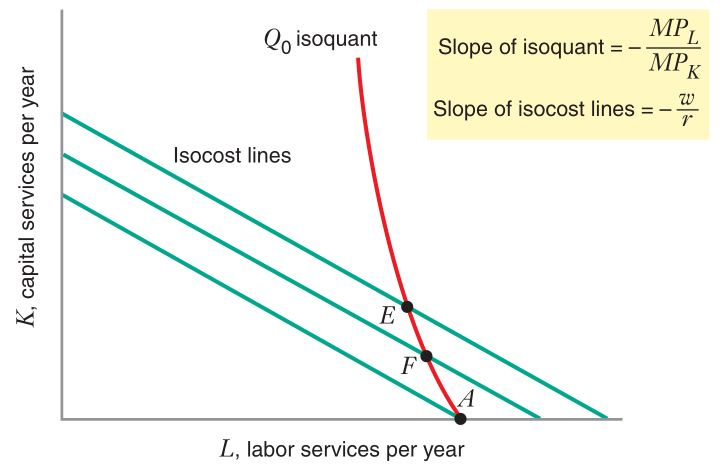
\includegraphics[width=0.7\linewidth]{figures/fig7_3.jpg}
  \end{figure}
\end{frame}

\begin{frame}{Corner Solutions}
  In these cases, the optimality condition won't hold

  \begin{itemize}
    \item Marginal product per dollar for one of the inputs will be strictly greater than the marginal product per dollar for the other.
    
    \item And cost is minimized by using all of that input.
  \end{itemize}

  \pause\bigskip 
  This is just like perfect substitutes in consumer choice!
\end{frame}

\begin{frame}
  \bgCranberry{Try It Yourself}

  \bigskip
  Suppose that for a firm that produces $\bar{Q}$ t-shirts, the cost of an hour of labor is \$5, and the cost of an hour of machine time is \$10. If at the current mix of labor and capital, a worker's output per hour is 15 t-shirts, and a machine's output is 25 t-shirts, which of the following is true?

  \bigskip
  \begin{enumerate}[A)]
    \item The firm should use more labor and less capital in order to reduce the cost of producing $\bar{Q}$ t-shirts.
    \item The firm should use more capital and less labor in order to reduce the cost of producing $\bar{Q}$ t-shirts.
    \item The firm is already producing $\bar{Q}$ t-shirts at the lowest cost.
    It's impossible to tell without knowing what $\bar{Q}$ is.
  \end{enumerate}
\end{frame}

\begin{frame}{Comparative Statics Analysis}
  Now that we have found the optimality condition for this problem, let's consider how the solution changes as our input prices and output quantity change.
  
  \bigskip
  Suppose that $w$ increases, with $r$ held constant. Then the optimal bundle becomes more expensive, and our optimality condition no longer holds. Now,
  $$
    \frac{MP_L}{w} < \frac{MP_K}{r}
  $$

  \pause 
  \begin{itemize}
    \item This means the firm gets more output per dollar from additional capital than from additional labor.
    
    \item And should use more capital and less labor.
  \end{itemize}
\end{frame}

\begin{frame}{Comparative Statics Analysis}
  Let's think about it another way. If the wage rate increases, then the slope of the isocost lines, $-\frac{w}{r}$, gets steeper.

  \pause
  \begin{itemize}
    \item The new point of tangency between the isocost and isoquant lines must be higher up on the isoquant.
    \item This implies that the firm will use more capital and less labor.
  \end{itemize}
\end{frame}

\begin{frame}{Comparative Statics Analysis}
  This diagram illustrates how, as the price of labor increases, the firm's optimal input combination is one with relatively more capital and less labor.

  \begin{figure}
    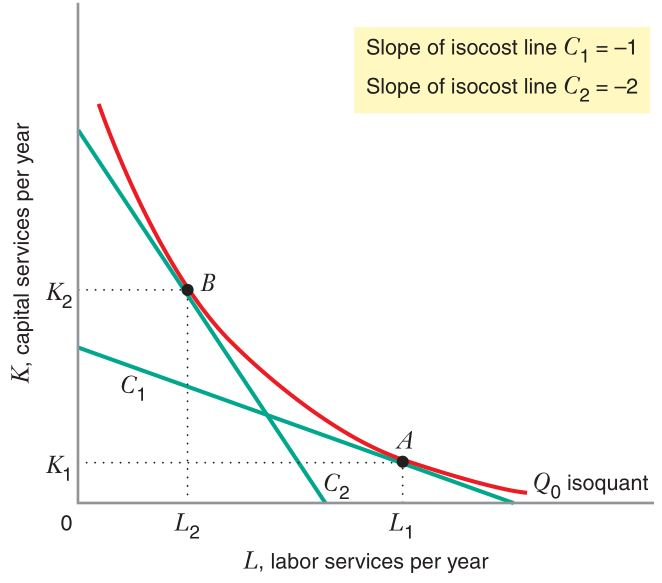
\includegraphics[width=0.5\linewidth]{figures/fig7_5.jpg}
  \end{figure}
\end{frame}

\begin{frame}{Comparative Statics Analysis}
  Now suppose the output quantity, $Q$, increases.

  \begin{itemize}
    \item Clearly, for the isoquant and isocost lines to remain tangent, the firm must move to a higher isocost (it costs more money to produce more output!)
    
    \item If we find the optimal bundle for a variety of output levels, we can trace what is called an \textbf{expansion path}
  \end{itemize}
\end{frame}

\begin{frame}{Normal and Inferior inputs}
  \begin{enumerate}
    \item If as the output quantity increases, demand for the input increases we say that the input is a \textbf{normal input}
    \item If as the output quantity increases, demand for the input decreases we say that the input is an \textbf{inferior input}
  \end{enumerate}

  \bigskip
  \emph{Note the similarities with quantity and income}
\end{frame}

\begin{frame}{Comparative Statics Analysis}
  Below is an expansion path where both inputs are normal inputs (as output increases, demand for both inputs increases)

  \begin{figure}
    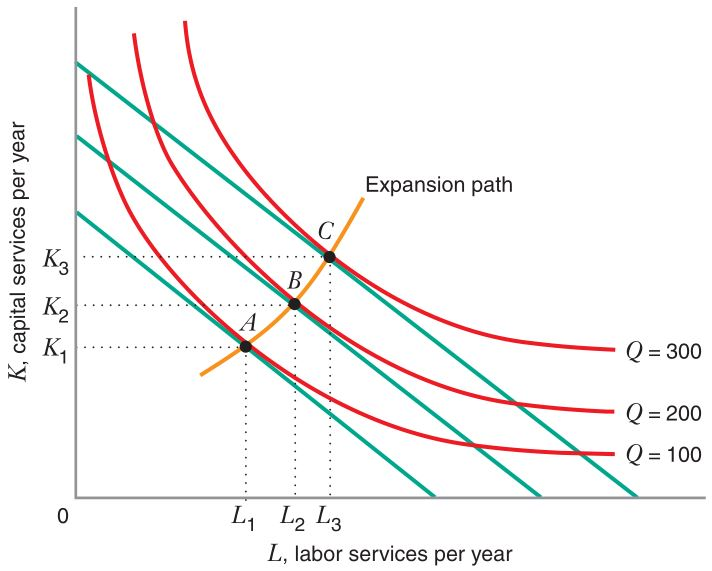
\includegraphics[width=0.6\linewidth]{figures/fig7_8.jpg}
  \end{figure}
\end{frame}

\begin{frame}{Comparative Statics Analysis}
  In this diagram, demand for labor decreases as quantity of output increases, implying that labor is an inferior input.

  \begin{figure}
    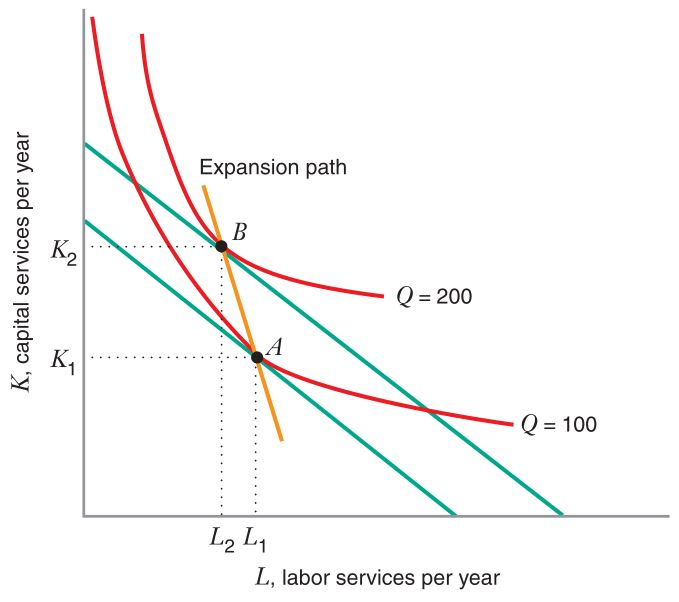
\includegraphics[width=0.6\linewidth]{figures/fig7_9.jpg}
  \end{figure}
\end{frame}

\begin{frame}{Comparative Statics}
  Suppose we want to do comparative statics numerically. For example, your boss asks you if they should buy more machines or hire more workers for their expanding business


  \begin{itemize}
    \item We can easily just solve for our conditional input demand functions, and plug in our old and new $w$, $r$, and $\bar{Q}$.
    
    \item Or, we can see how the functions vary as we change an input using partial derivatives.
  \end{itemize}
\end{frame}

\begin{frame}{Comparative Statics and Partial Derivatives }
  From above, we had 
  $$
    L^*(w,r,\bar{Q}) = \frac{\bar{Q}}{50} \sqrt{\tfrac{r}{w}}
  $$

  \bigskip
  Then 
  $$
    \frac{\partial L^*(w,r,\bar{Q})}{\partial w} = -\frac{\bar{Q}}{25} \sqrt{\frac{r}{w^3}} 
  $$
\end{frame}

\begin{frame}
  \bgCranberry{Try It Yourself}

  \bigskip
  Which of the following conditional factor demand functions represents demand for an \textit{inferior} input?

  \bigskip
  \begin{enumerate}[A)]
    \item $L(w,r,Q) =  10\frac{w}{rQ}$

    \item $L(w,r,Q) =  10(w + rQ)$

    \item $L(w,r,Q) =  10\frac{wQ}{r}$

    \item $L(w,r,Q) =  10\frac{Q}{wr}$
  \end{enumerate}
\end{frame}

\begin{frame}{Price Elasticity of Input Demand}
  In chapter 2, we learned how to describe the sensitivity of demand for a good to a change in the price. The same principle can be applied with input demand.

  \bigskip
  The \textbf{price elasticity of demand for labor} is given by

  \begin{equation*}
    \epsilon_{L,w}=\frac{\frac{\Delta L}{L}\times 100\%}{\frac{\Delta w}{w} \times 100 \%} = \frac{\Delta L}{\Delta w}\frac{w}{L}
  \end{equation*}

  \pause\bigskip
  The \textbf{price elasticity of demand for capital} is given by

  \begin{equation*}
    \epsilon_{K,r}=\frac{\frac{\Delta K}{K}\times 100\%}{\frac{\Delta r}{r} \times 100 \%} = \frac{\Delta K}{\Delta r}\frac{r}{K}
  \end{equation*}
\end{frame}

\begin{frame}{Price Elasticity of Input Demand}
  Remember that an elasticity measures the percentage change in demand for an input that results from a 1\% change in some price.

  \begin{itemize}
    \item That means that if labor has a price elasticity of $3$, then if the wage increases by 1\%, demand for labor will decrease by $3\%$.
  \end{itemize}
  
  \pause\bigskip
  If we have input demand functions, then our price elasticity can be calculated using the derivative:

  \vspace*{-5mm}
  \begin{align*}
    \epsilon_{L,w} &= \frac{\Delta L}{\Delta w}\frac{w}{L} = \frac{\partial L}{\partial w}\frac{w}{L} \\
    \epsilon_{K,r} &= \frac{\Delta K}{\Delta r}\frac{r}{K} = \frac{\partial K}{\partial r}\frac{r}{K}
  \end{align*}
\end{frame}

\begin{frame}{Price Elasticity of Input Demand}
  Price elasticity of input demand depends, in part, on the elasticity of substitution.

  \bigskip 
  Suppose that a firm can more easily substitute capital for labor.
  \begin{itemize}
    \item Then if the price of labor increases slightly, they will use more capital and less labor.
  \end{itemize}

  \pause\bigskip
  On the other hand, if capital and labor are complements for a firm...
  \begin{itemize}
    \item Their mix of capital and labor may not change much in response to a change in the wage.
  \end{itemize}
\end{frame}

\begin{frame}{Price Elasticity of Input Demand}
  \begin{figure}
    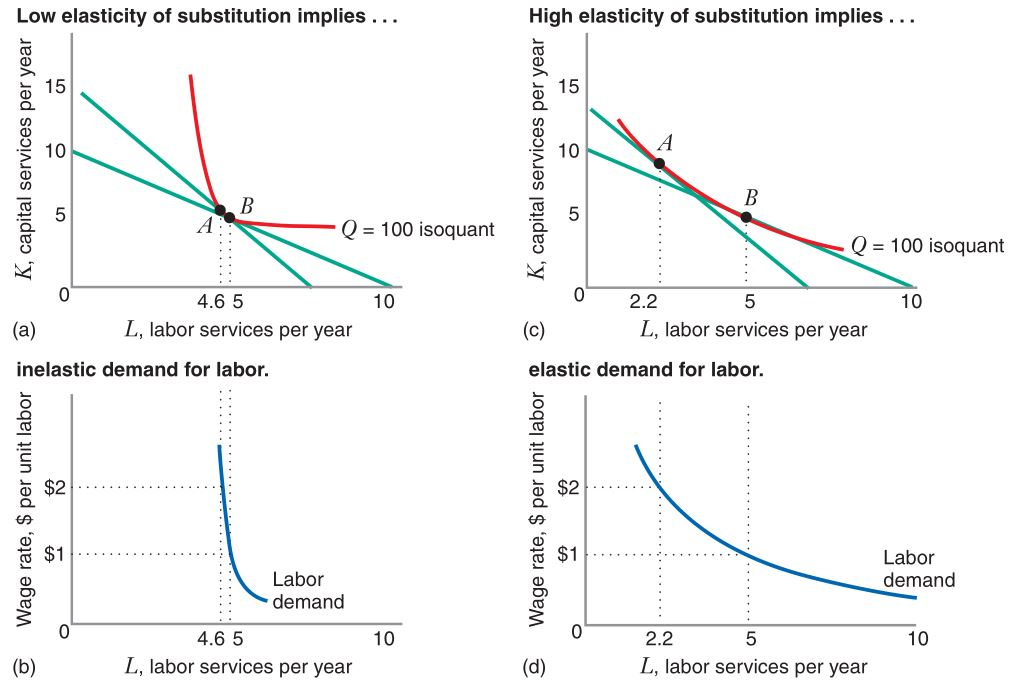
\includegraphics[width=0.9\linewidth]{figures/fig7_11.jpg}
  \end{figure}
\end{frame}

\begin{frame}{Price Elasticity of Input Demand}
  These elasticities are important for policy decisions. For example, what will the impact on labor demand be if the government increases the minimum wage?
  
  \begin{itemize}
    \item If the wage elasticity of labor demand is low, then firms will still hire almost as many workers as before. 
    
    \item But if the wage elasticity of labor demand is high, they may substitute to capital instead (like self-checkout machines).
  \end{itemize}
\end{frame}

\begin{frame}
  \bgCranberry{Try It Yourself}

  \bigskip
  Suppose that the price of low-skill labor increases as a result of an increase in the federal minimum wage. Assume that firms cannot adjust their level of output. For which type of firm will total cost be impacted the most?

  \bigskip
  \begin{enumerate}[A)]
    \item A retail store such as Target, for whom cashiers and self-checkout stations are substitutes.
    \item A graphic design firm, for whom designers and computers are complements.
  \end{enumerate}
\end{frame}

\begin{frame}{Fixed and Variable Costs}
  A firm's costs can be divided into two types:

  \begin{enumerate}
    \item \textbf{Fixed costs} refer to costs that do not vary with the level of output.
    
    \begin{itemize}
      \item For example, a nail salon might have to pay rent every month, regardless of whether they have no customers, or 1,000 customers.
    \end{itemize}
    
    \item \textbf{Variable costs} refer to costs that depend on the level of output.
  
    \begin{itemize}
      \item For example, a bakery's quantity of output depends on how many hours their bakers work.
    \end{itemize}
  \end{enumerate}
\end{frame}

\begin{frame}{Fixed and Variable Costs}
  The total cost function is a sum of the two costs:
  
  \begin{enumerate}
    \item \textbf{Total variable cost} is made up of all of the firm's expenditures on variable inputs, such as labor and materials.
    \item \textbf{Total fixed cost} is made up of all expenditures that do not vary with output.
  \end{enumerate}
\end{frame}

\begin{frame}{Sunk Costs}
  When it comes to fixed costs, some can be avoided if the firm chooses not to produce (e.g. lighting for an office building).

  \bigskip
  But some cannot be recovered even if a firm shuts down (e.g. license fees or a very specialized piece of equipment).

  \begin{itemize}
    \item Fixed costs that cannot be recovered or avoided are known as \textbf{sunk costs}.
  
    \item Fixed costs that can be recovered, or are avoidable in the event that the firm does not produce, are known as \textbf{nonsunk costs}.
  \end{itemize}
\end{frame}

\begin{frame}{Sunk Costs}
  In general, sunk costs are irrelevant to a firm's decisions. If the cost cannot be recovered, then whether the firm continues producing (and if so, how much), do not depend on that cost.

  \begin{itemize}
    \item However, if the sunk cost has not yet been paid, it is relevant.
    
    \item A firm can decide whether or not to incur the cost in the first place.
  \end{itemize}
\end{frame}

\begin{frame}{Short-Run vs. Long-Run}
  Until this point, we've really only considered the long run.

  \begin{itemize}
    \item The \textbf{long run} refers to a time period over which all inputs can vary (capital and labor).
    \item In the \textbf{short run}, at least one input is fixed.
  \end{itemize}

  \bigskip
  Usually we assume capital is fixed (e.g. rent on a building). \pause But it could also be labor (maybe firms hire employees on a 1-year contract).
\end{frame}

\begin{frame}{Cost Minimization in the Short Run}
  In the short run, a firm's total cost will always be greater than or equal to a firm's long-run total cost.

  \begin{itemize}
    \item Because if it were lower in the short run, they would use that same input combination in the long run.
  \end{itemize}

  \pause\bigskip
  Suppose for example that capital is fixed at $\bar{K}$ units.

  \begin{itemize}
    \item Then in the short run, the firm may not be able to achieve the cost-minimizing input combination, so costs will be higher.
  \end{itemize}
\end{frame}

\begin{frame}{Cost Minimization in the Short Run}
  Because capital is fixed, the firm's lowest-cost input combination leaves them at a higher isocost line than the long-run cost-minimizing input combination (F in the short-run; A in the long-run)

  \begin{figure}
    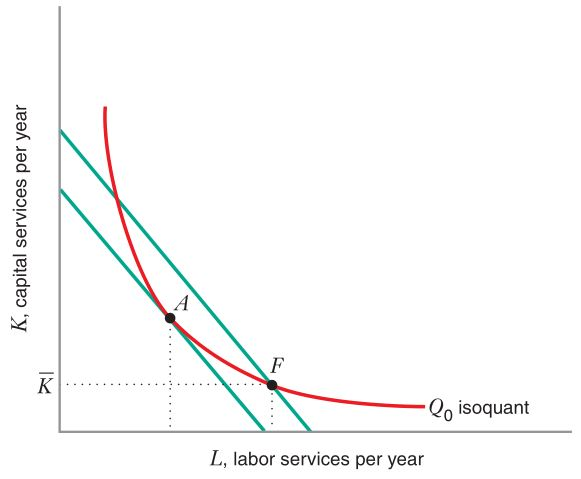
\includegraphics[width=0.6\linewidth]{figures/fig7_13.jpg}
  \end{figure}
\end{frame}

\begin{frame}{Cost Minimization in the Short Run}
  What about our optimality condition?

  \begin{itemize}
    \item You can see from the previous diagram that at the  short-run cost minimizing point, our isoquant and isocost lines are no longer tangent.
    
    \item Our optimality condition doesn't hold.
  \end{itemize}

  \pause\bigskip
  Let's try to find the cost-minimizing point using calculus.
\end{frame}

\begin{frame}{Cost Minimization in the Short Run}
  Suppose a firm's production function is given by $Q =50\sqrt{KL}$. In the short-run, the firm's problem becomes

  $$
    \min_{L} wL+ r\bar{K} \qquad \text{subject to} \qquad \bar{Q} = 50\sqrt{\bar{K}L}
  $$

  \pause\bigskip
  Note that, because K is fixed, we only have 1 choice variable. In this case, we now simply have 1 equation, $\bar{Q} = 50\sqrt{\bar{K}L}$), and 1 unknown, $L$.
  
  \bigskip
  We can then simply solve for $L$.
  \begin{equation*}
    L^*(w,r,\bar{Q}) = \frac{\bar{Q^2}}{(2500\bar{K})}
  \end{equation*}
\end{frame}

\begin{frame}
  \bgCranberry{Try It Yourself}

  \bigskip
  Suppose that a firm has the following production function: $Q(K,L)=15KL$. In the short run, suppose that $K$ is fixed at $\bar{K}=5$. If a cost-minimizing firm decides to produce $Q=1500$ units, find the cost-minimizing level of labor.

  \bigskip
  \begin{enumerate}[A)]
    \item 5 units
    \item 10 units
    \item 15 units
    \item 20 units
  \end{enumerate}
\end{frame}

\begin{frame}{Comparative Statics}
  What if the output quantity changes?

  \begin{itemize}
    \item Well, in the short run, $K$ is still fixed, so the firm can only vary the amount of labor used.
    
    \item This results in a short-run expansion path that's horizontal.
    
    \item In the long run, however, both inputs can vary, resulting in a different long-run expansion path.
  \end{itemize}


\end{frame}

\begin{frame}{Comparative Statics}
  Below are the short-run and long-run expansion paths for a production function.

  \begin{figure}
    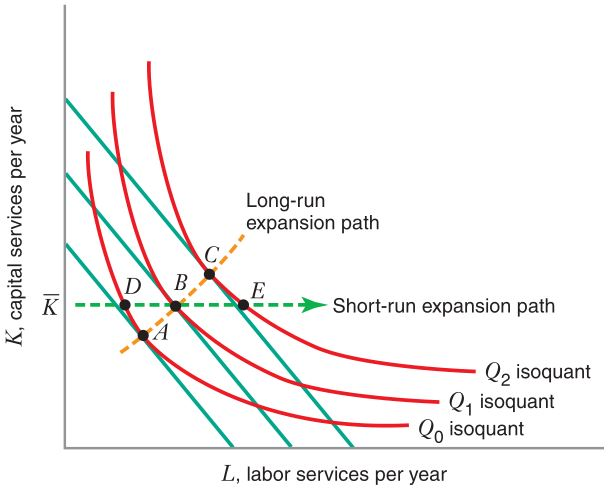
\includegraphics[width=0.6\linewidth]{figures/fig7_14.jpg}
  \end{figure}
\end{frame}
\end{document}

